\documentclass[border=3pt]{standalone}
% Preâmbulo compartilhado pelos diagramas TikZ da aula 4 de Navegação (Representação de Mapas)
\usepackage[T1]{fontenc}
\usepackage[utf8]{inputenc}
\usepackage{lmodern}
\usepackage{amsmath}
\usepackage{xcolor}
\usepackage{tikz}
\usetikzlibrary{arrows.meta,angles,quotes,decorations.pathmorphing,decorations.pathreplacing,calc,
                positioning,shapes.geometric,shapes.misc,backgrounds,fit,
                math}

% Paleta (mesma dos SVGs originais)
\definecolor{dblue}{HTML}{2A5B8C}
\definecolor{dorange}{HTML}{B3541E}
\definecolor{dgreen}{HTML}{4A7C59}
\definecolor{dred}{HTML}{9C4B4B}
\definecolor{dcream}{HTML}{F4F1EA}
\definecolor{dshade}{HTML}{DDD7C9}

% Função gaussiana (não normalizada por padrão de escala visual)
\pgfmathdeclarefunction{gauss}{3}{%
  \pgfmathparse{1/(#3*sqrt(2*pi))*exp(-((#1-#2)^2)/(2*#3^2))}%
}

% Estilos comuns (prefixo d... para não colidir com chaves internas do pgf)
\tikzset{
  >={Stealth[length=2mm]},
  dguide/.style={gray!55, dashed, line width=0.4pt},
  daxis/.style={gray!60, line width=0.7pt, ->},
  dbody/.style={fill=black!3, draw=black!80, line width=1pt},
  dacc/.style={draw=dblue, line width=1pt},
  dlbl/.style={black!55, font=\small},
  dsub/.style={black!45, font=\footnotesize},
  dstate/.style={circle, draw=black!80, fill=dcream, line width=1pt,
                 minimum size=17mm, font=\large, inner sep=1pt},
  dobs/.style={circle, draw=black!80, fill=dshade, line width=1pt,
               minimum size=14mm, font=\large, inner sep=1pt},
  dbox/.style={rounded corners=2pt, draw=black!80, fill=dcream, line width=1pt,
               align=center, inner sep=6pt},
  dop/.style={circle, draw=black!80, fill=white, line width=1pt,
              minimum size=6mm, inner sep=0pt, font=\small},
  dtrans/.style={->, dblue, line width=1pt},
  dmeas/.style={->, dorange, line width=1pt},
  dcurve/.style={line width=1pt, dblue},
  dcurveb/.style={line width=1.4pt, dorange},
}

\begin{document}
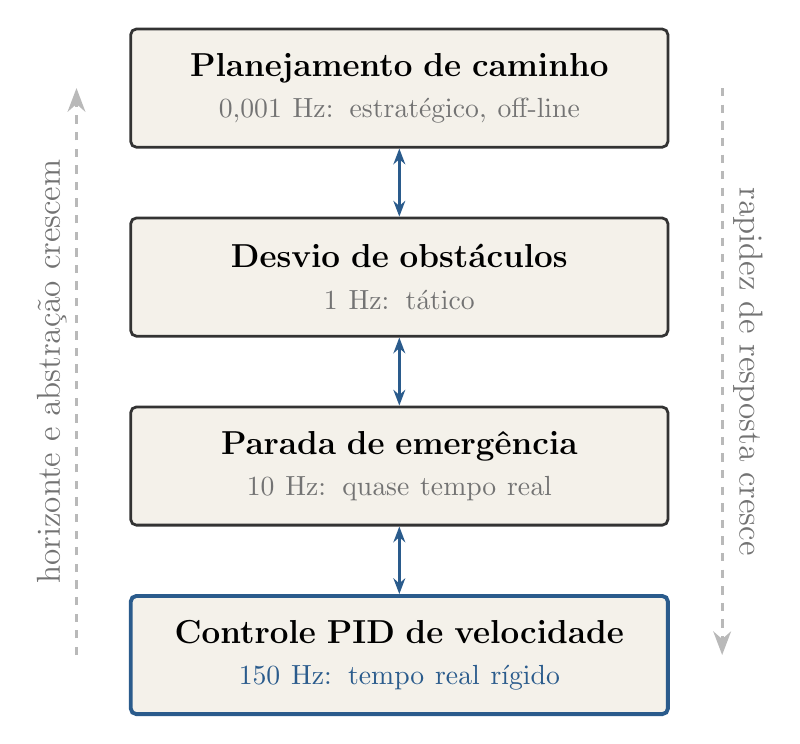
\begin{tikzpicture}[x=1cm,y=1cm]

  \tikzset{mod/.style={dbox, text width=6.4cm, minimum height=1.5cm, font=\large, align=center}}
  \node[mod] (n1) at (0,7.2) {\textbf{Planejamento de caminho}\\[1pt]{\normalsize\color{black!55}0{,}001 Hz: estratégico, off-line}};
  \node[mod] (n2) at (0,4.8) {\textbf{Desvio de obstáculos}\\[1pt]{\normalsize\color{black!55}1 Hz: tático}};
  \node[mod] (n3) at (0,2.4) {\textbf{Parada de emergência}\\[1pt]{\normalsize\color{black!55}10 Hz: quase tempo real}};
  \node[mod, draw=dblue, line width=1.4pt] (n4) at (0,0) {\textbf{Controle PID de velocidade}\\[1pt]{\normalsize\color{dblue}150 Hz: tempo real rígido}};

  \draw[dtrans, <->] (n1.south) -- (n2.north);
  \draw[dtrans, <->] (n2.south) -- (n3.north);
  \draw[dtrans, <->] (n3.south) -- (n4.north);

  \draw[dguide, line width=1.2pt, -{Stealth[length=3mm]}] (-4.1,0) -- (-4.1,7.2) node[midway, sloped, above, dlbl, font=\large] {horizonte e abstração crescem};
  \draw[dguide, line width=1.2pt, -{Stealth[length=3mm]}] (4.1,7.2) -- (4.1,0) node[midway, sloped, above, dlbl, font=\large] {rapidez de resposta cresce};

\end{tikzpicture}
\end{document}
